\chapter{Some Big Ideas}

\includegraphics[scale=0.85]{../images/book-5104342_1920.jpg}

\justify
There are some key concepts, tenets, and precepts that will serve the aspiring DevSecOps engineer well. In this chapter we will explore some of these to levelset our understanding and introduce the reader to the vernacular of the modern day software engineer in a world gone cloudy.

\section{The Flow (a.k.a. Pipelines)}

\justify
Work products such as code and documents begin their life on developer workstations. In this book we will refer to the environments where this takes place as the "local" environment. These work products are created, reviewed and checked into Revision Control Systems (RCS)\index{Revsion Control System (RCS)}, GitHub\index{GitHub} for example, by the DevSecOps practitioner. Other revison control systems include GitLab\index{GitLab} and BitBucket\index{BitBucket}.

\justify
Test cases are created and run against the work products at check-in time, to ensure stability, security, and compatibility with the existing code base. The automation required to execute tests every time work is checked in is also typically the responsibility of the DevSecOps engineers. As seen in figure \ref{fig:pipeline}, work typically "flows" from the local environments, into a test environment, and finally to production where
it is available for use by the entire user base.

\begin{figure}[!htb]
	\centering
	\includegraphics[scale=0.63]{../images/flow.png}
	\caption{Typical build pipeline.}
	\label{fig:pipeline}
\end{figure}

\justify
We will refer to the entirety of this three-stage flow as one example of
a "pipeline"\index{pipeline}. Code from one or more local environments is checked in to
the revision control system throughout a typical DevSecOps workday, and
continuously tested and integrated with the main code base. That is to
say, work undergoes "Continuous Integration" (CI)\index{Continuous Integration (CI)} with the main code base, and often "Continuous Delivery" (CD)\index{Continuous Delivery (CD)} between local, test, and production environments. This is where the term "CI/CD Pipeline" comes from.

\justify
While the CI/CD Pipeline is often the primary focus of the DevSecOps engineer, other pipelines exist as well. For example, let's assume our organization maintains a vast pool of raw data, also known as a data
lake\index{Data Lake}. The staff Data Engineers build and maintain Data Science\index{Data Science} pipelines
to facilitate the smooth flow of logs and other data into that data lake. Now Data Scientists are able to create machine learning models that rely on that data to produce useful insights. As another example,
consider code changes as they move from developer workstations into a code repository for storage. Accessing this code for the purpose of testing will differ from how it is accessed for the purposes of
deployment. The order of operations and flow between differing functions might be said to comprise two different pipelines.

\section{Shifting Left}

\justify
We now have a mental picture of how software will flow from Development, to Test, and to Production. Integration security into this flow, as early and as often as possible, is highly desirable. Imagine our software life cycle occurring along a temporal axis, t. Intentionally moving security to the left on this axis (lower values of t) is known as "Shifting Left"\index{Shift Left} as seen in figure \ref{fig:shift}.

\begin{figure}[!htb]
	\centering
	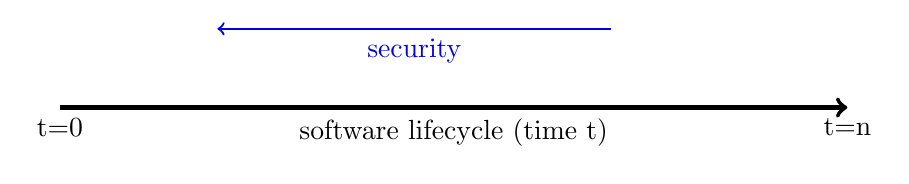
\begin{tikzpicture}
	  \draw[<-,thick,black!10!blue](2.0cm,\nOne) -- (7.0cm,\nOne) node[midway,below]{security};
	  \draw [->, ultra thick] (0,0) -- (10,0) node[pos=0, below]{t=0} node[pos=0.5,below]{software lifecycle (time t)} node[pos=1, below]{t=n};
	\end{tikzpicture}\\
	\caption{Shifting security to the left.}
	\label{fig:shift}
\end{figure}

\section{Automation}

\justify
Consider what may happen when we want to apply the lessons from this book across a large environment made up of many hosts, containers, pieces of application software, etc. It becomes a huge challenge for an operator to log in to each host or container individually. Typing, or even cutting and pasting commands to keep things up and running properly, look at logs, and so on becomes problematic. Creating shell scripts can be quite helpful, but is an outdated modality when we consider the daunting size and complexity of the modern administrative domain.

\justify
This is where automation comes in. Automation\index{automation} is a way to provision and maintain some or many hosts in a programmatic manner. Another desirable goal, and hopefully result of automation is to reduce the amount of per-host interaction that comes with the work of administering systems. Automation is the force multiplier we use to achieve scaling\index{scaling}. Couple this precept with the explosive automation tooling ecosystem and you are on the path to doing more, better work in less time with a smaller staff. 

\section{Ephemerality}

\justify
Ephemerality/index{Ephemerality} is the concept of something being transitory in nature,
existing only briefly\footnote{\url{https://en.wikipedia.org/wiki/Ephemerality}}.
Using immutable containers makes it easier to realize infrastructure and
hosts that are ephemeral. Rather than spending a great deal of time
patching and upgrading one or more hosts as we might in a traditional
project stack that uses virtual machines or bare metal, we're going to
use Docker to create a new container in place of the old one. In other
words, we're running our project in containers that are immutable and
ephemeral to the degree possible.

\section{Immutability}

\justify
There is obvious advantage of being able to quickly stand up new clones
of our project to replace existing instances that may be outdated,
insecure, etc. The idea of immutability\footnote{\url{https://www.hashicorp.com/resources/what-is-mutable-vs-immutable-infrastructure/}},
in reference to software projects, is the degree to which something, our
running project for example, can be changed. Immutability\index{Immutability} is desirable,
in that we wish to be able to simply replace outdated instances of our
project in their entirety. Upgrading and patching are inherently
problematic activities, high cost in terms of time, effort and money,
that we have the technology to dissociate from. With containerization,
we can more easily achieve immutability across the software life cycle.

\section{Agile Methodologies}

\justify
The concept of Agile\index{agile} Software development is an expansive topic unto itself. Although we won't implicitly dedicate a lot of our time to these ideas, agile is widely regarded as an underpinning of a successful
DevSecOps program.